\subsection{CNN Results and Comparison with MC-NNM}

\begin{figure}[htbp]
    \centering
        \begin{subfigure}[c]{0.45\textwidth}
        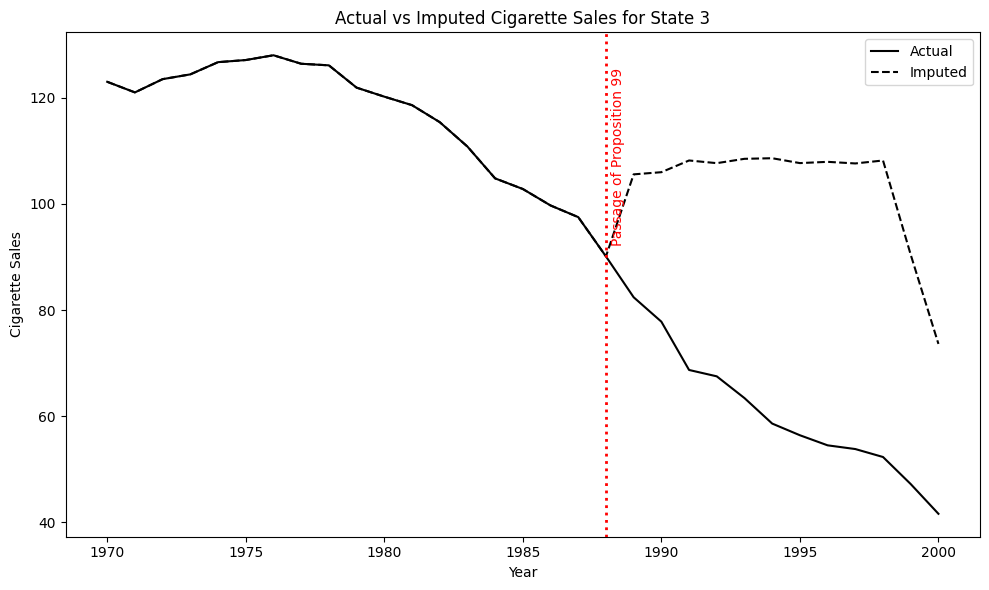
\includegraphics[width=\textwidth]{../figures/cnn-1.png}
        \caption{CNN}
        \label{fig:cnn}
    \end{subfigure}
    \begin{subfigure}[c]{0.45\textwidth}
        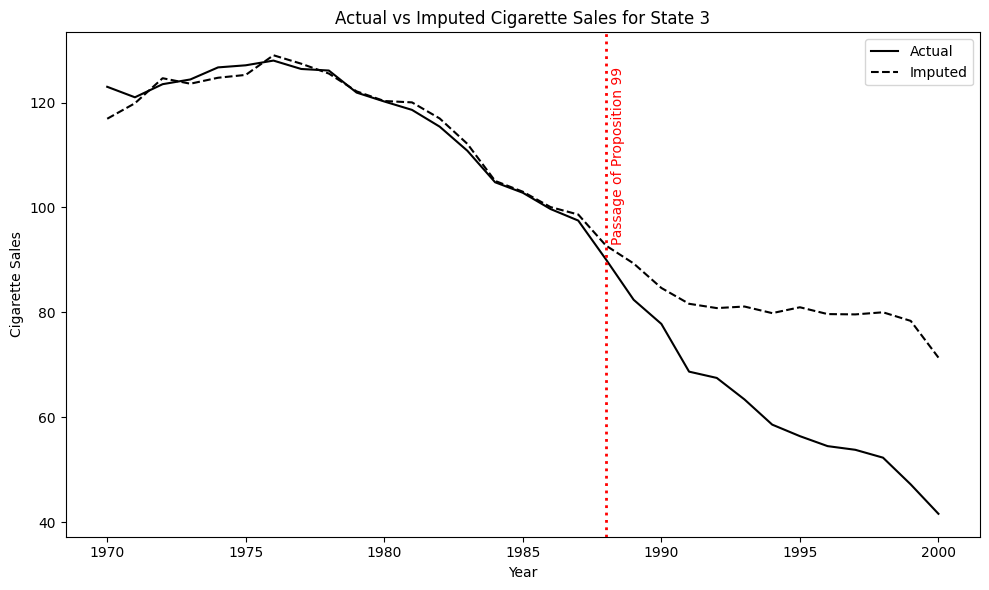
\includegraphics[width=\textwidth]{../figures/mc-nnm-1.png}
        \caption{MC-NNM }
        \label{fig:mcnnm}
    \end{subfigure}
    \caption{Counterfactuals for California Proposition 99 Data}
    \label{fig:main_results}
    \begin{minipage}{0.9\textwidth}
        \scriptsize
        \textbf{Notes:} The left panel shows the CNN counterfactuals, while the right panel shows the MC-NNM counterfactuals for California's cigarette sales data. The horizontal red dashed lines indicate the treatment period. The solid black lines represent the actual outcomes of the treated unit, and the dashed lines represent the predicted counterfactual outcomes.
        In terms of \textcite{rubin1974estimating}'s framework, the gap between the solid and dashed lines represents the estimated treatment effect.
    \end{minipage}
\end{figure}

Figure \ref{fig:main_results} displays the actual and counterfactual outcomes
of California's cigarette sales using CNN and MC-NNM methods.
Subtracting the imputed counterfactuals from the actual outcomes yields the estimated treatment effect of Proposition 99, which is shown as the gap between the solid and dashed lines in Figure \ref{fig:main_results}.
Compared to the MC-NNM results, the CNN counterfactuals were less smooth, and possibly more sensitive to the 
peculiarities of the data.
In terms of direction, both methods produced similar counterfactuals (i.e., both predicted a decrease in cigarette sales after the implementation of Proposition 99),
but the CNN counterfactuals were more volatile, especially in the beginning and the end of the post-treatment periods.

Such sudden surge and drop in the CNN counterfactuals may reflect zero paddings and the convolutional nature of the CNN model,
suggesting that calibration must be done carefully before applying CNNs to panel data.




\subsection{Placebo Tests}

\begin{figure}[htbp]
    \centering
    \begin{subfigure}[c]{0.3\textwidth}
        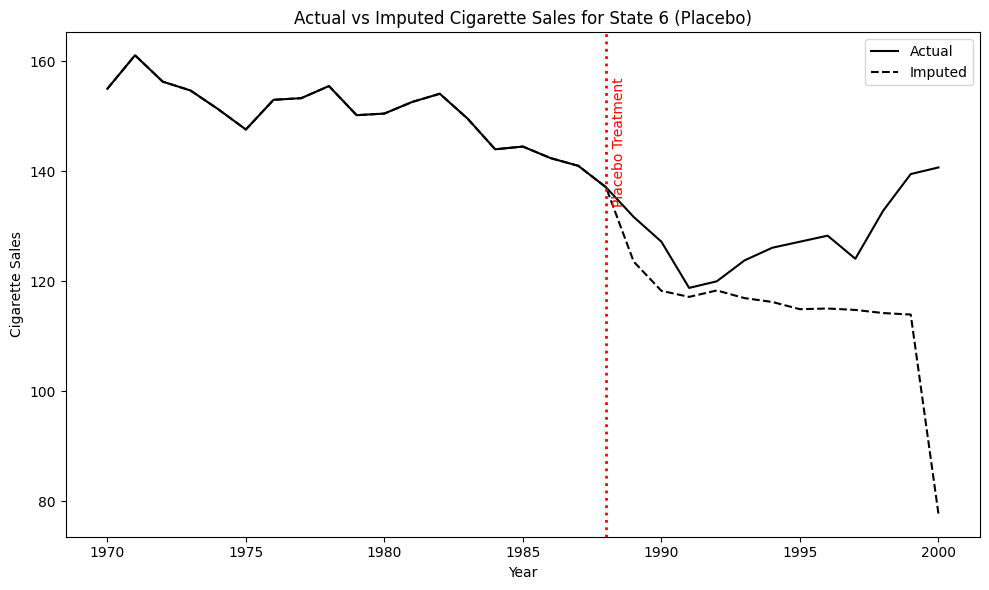
\includegraphics[width=\textwidth]{../figures/cnn-2.png}
        \caption{Delaware}
        \label{fig:placebo_1}
    \end{subfigure}
    \begin{subfigure}[c]{0.3\textwidth}
        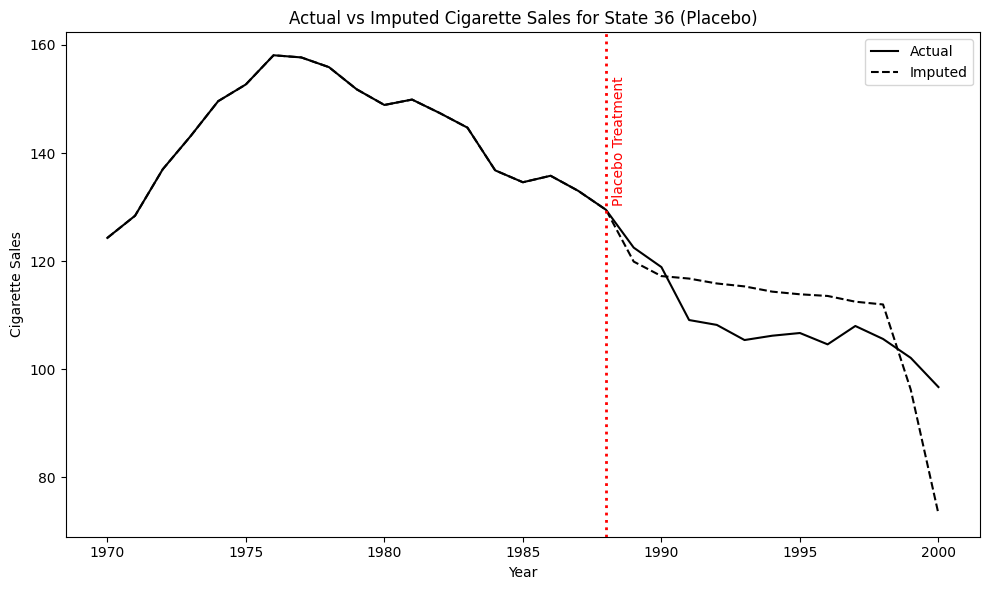
\includegraphics[width=\textwidth]{../figures/cnn-3.png}
        \caption{Virginia}
        \label{fig:placebo_2}
    \end{subfigure}
    \begin{subfigure}[c]{0.3\textwidth}
        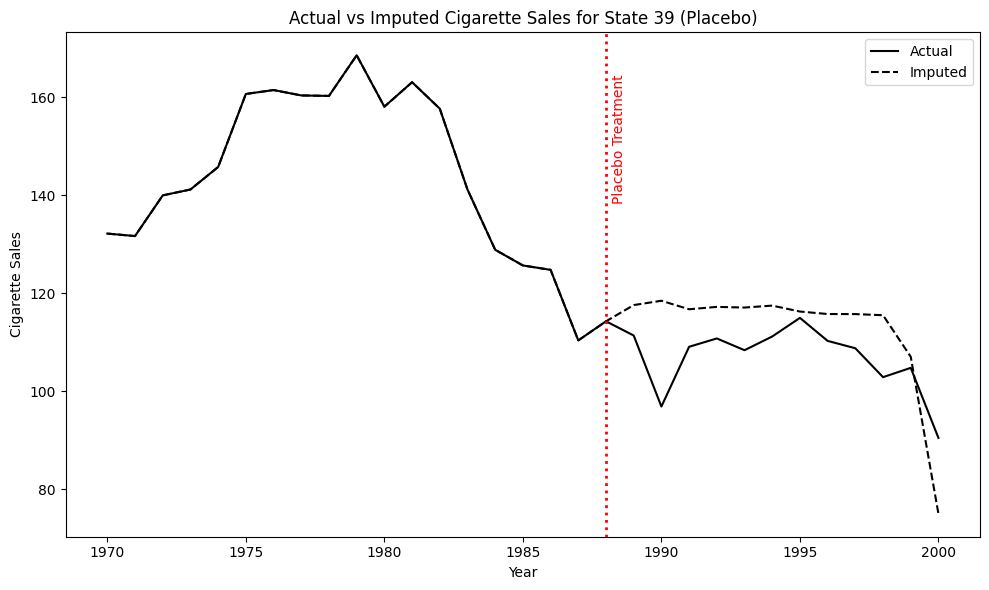
\includegraphics[width=\textwidth]{../figures/cnn-4.png}
        \caption{Wyoming}
        \label{fig:placebo_3}
    \end{subfigure}
    \caption{Placebo Test: CNN Counterfactuals for California Proposition 99 Data}
    \label{fig:placebo_cnn}
\end{figure}


\begin{figure}[htbp]
    \centering
    \begin{subfigure}[c]{0.3\textwidth}
        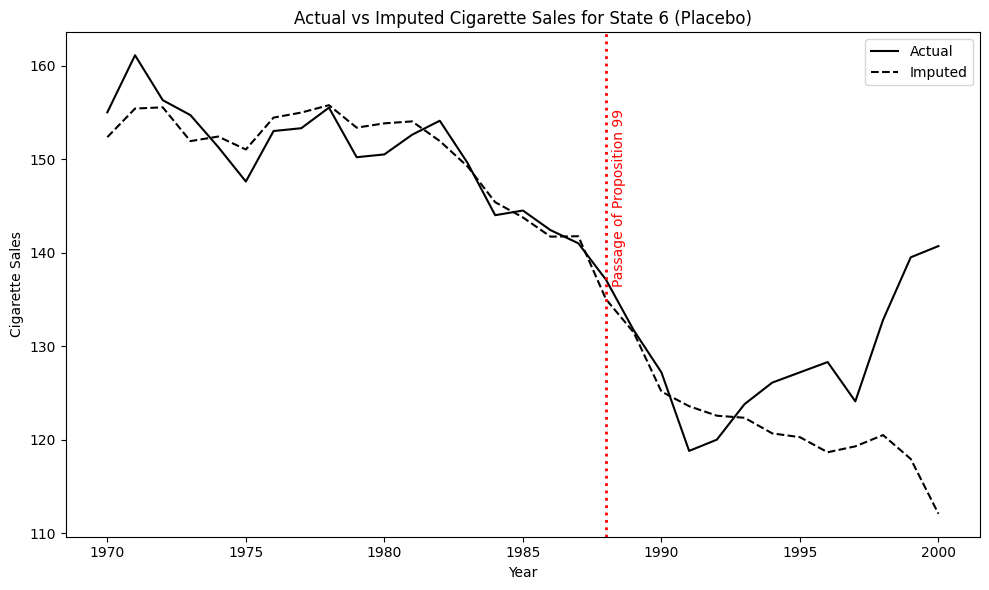
\includegraphics[width=\textwidth]{../figures/mc-nnm-2.png}
        \caption{Delaware}
        \label{fig:placebo_1}
    \end{subfigure}
    \begin{subfigure}[c]{0.3\textwidth}
        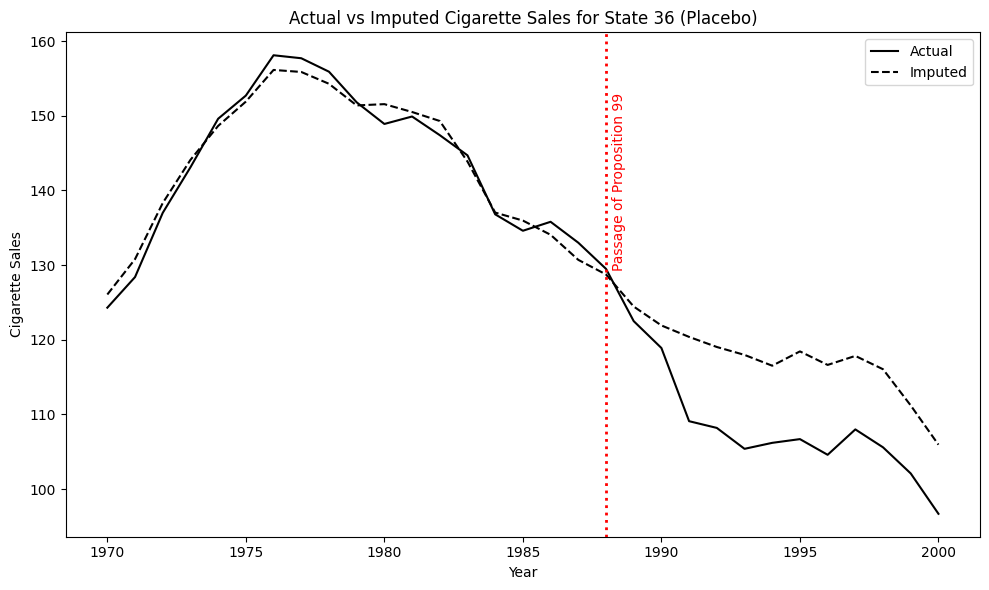
\includegraphics[width=\textwidth]{../figures/mc-nnm-3.png}
        \caption{Virginia}
        \label{fig:placebo_2}
    \end{subfigure}
    \begin{subfigure}[c]{0.3\textwidth}
        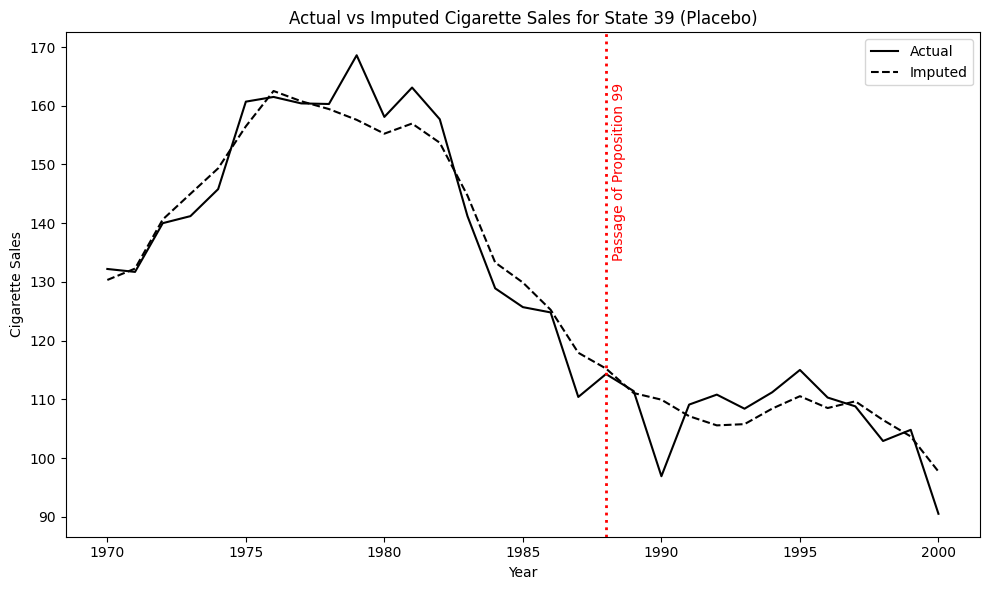
\includegraphics[width=\textwidth]{../figures/mc-nnm-4.png}
        \caption{Wyoming}
        \label{fig:placebo_3}
    \end{subfigure}
    \caption{Placebo Test: MC-NNM Counterfactuals for California Proposition 99 Data}
    \label{fig:placebo_mcnnm}
\end{figure}

To further validate the counterfactual predictions, we conducted placebo tests by applying the CNN and MC-NNM methods to the data, but treating other states as if they were the treated unit and excluding California.
Figures \ref{fig:placebo_cnn} and \ref{fig:placebo_mcnnm} show the results of these placebo tests for CNN and MC-NNM, respectively.


In these figures, we observe that both CNN and MC-NNM methods produce similar predictions for the placebo states and match the actual outcomes closely - reflecting the null treatment effect in these states.
Two patterns are worth noting: first, when MC-NNM does not perform well, CNN fails as well (see Delawre);
second, CNN tends to produce more volatile results at the end of the time series, which reflects the zero padding.
